\chapter{Cuádricas}
\section{Definición}
Nos interesan las superficies de ecuación $z=f(x, y)$ o $F(x, y, z)=0$, es decir, las superficies formadas por los puntos $(x, y, z)$ que satisfacen la ecuación $z=f(x, y) \circ F(x, y, z)=0$.

En particular trabajaremos únicamente con superficies cuádricas cuyas ecuaciones están dadas en forma canónica.

Existen seis tipos básicos de superficies cuádricas: Elipsoide, Hiperboloide de una hoja, Hiperboloide de dos hojas, Cono Elíptico, Paraboloide Elíptico y Paraboloide Hiperbólico. \cite{solis2016graficas}.
\subsection{Elipsoide}
Ecuación canónica:
$$
    \frac{(x-i)^{2}}{a^{2}}+\frac{(y-j)^{2}}{b^{2}}+\frac{(z-k)^{2}}{c^{2}}=1
$$
Parametrización:
$$
    s(u, v):\left\{\begin{array}{l}
        x=i-a \cos u \operatorname{sen} v                 \\
        y=j-b \operatorname{sen} u \operatorname{sen} v ; \\
        z=k-c \cos v
    \end{array} \quad u \in[0,2 \pi], v \in[0, \pi]\right.
$$

\subsection{Hiperboloide de una hoja}
Ecuación canónica:
$$
    \frac{(x-i)^{2}}{a^{2}}+\frac{(y-j)^{2}}{b^{2}}-\frac{(z-k)^{2}}{c^{2}}=1
$$
Parametrización:
$$
    s(u, v):\left\{\begin{array}{l}
        x=i-a \cos u \cosh v                 \\
        y=j-b \operatorname{sen} u \cosh v ; \\
        z=k-c \operatorname{senh} v
    \end{array} \quad u \in[0,2 \pi], v \in \mathbb{R}\right.
$$

\subsection{Hiperboloide de dos hoja}
Ecuación canónica:
$$
    -\frac{(x-i)^{2}}{a^{2}}-\frac{(y-j)^{2}}{b^{2}}+\frac{(z-k)^{2}}{c^{2}}=1
$$
Parametrización:
$$
    s(u, v):\left\{\begin{array}{l}
        x=i+a \senh u \cos v                 \\
        y=j+b \operatorname{senh} u \sen v ; \\
        z=k+c \operatorname{cosh} u
    \end{array} \quad u \in[0, + \infty], v  \in[0,2 \pi] \right.
$$

\subsection{Cono elíptico centrado}
Ecuación canónica:
$$
    \frac{(x-i)^{2}}{a^{2}}+\frac{(y-j)^{2}}{b^{2}}-\frac{(z-k)^{2}}{c^{2}}=0
$$
Parametrización:
$$
    s(u, v):\left\{\begin{array}{l}
        x=i+\frac{a}{c} \operatorname{senh} u \cos v                 \\
        y=j+\frac{b}{c} \operatorname{senh} u \operatorname{sen} v ; \\
        z=k+\operatorname{senh} u
    \end{array} \quad u \in \mathbb{R}, v \in[0,2 \pi]\right.
$$

\subsection{Paraboloide elíptico}
Ecuación canónica:
$$
    z-k=\frac{(x-i)^{2}}{a^{2}}+\frac{(y-j)^{2}}{b^{2}}
$$
Parametrización:
$$
    s(u, v):\left\{\begin{array}{l}
        x=u \\
        y=v \\
        z=\frac{(u-i)^{2}}{a^{2}}+\frac{(v-j)^{2}}{b^{2}}+k
    \end{array} ; \quad u \in \mathbb{R}, v \in \mathbb{R}\right.
$$

\subsection{Paraboloide Hiperbólico}
Ecuación canónica:
$$
    z-k=-\frac{(x-i)^{2}}{a^{2}}+\frac{(y-j)^{2}}{b^{2}}
$$
Parametrización:
$$
    s(u, v):\left\{\begin{array}{l}
        x=u \\
        y=v \\
        z=-\frac{(u-i)^{2}}{a^{2}}+\frac{(v-j)^{2}}{b^{2}}+k
    \end{array} ; \quad u \in \mathbb{R}, v \in \mathbb{R}\right.
$$
\subsection{Ejemplo}

Considere el elipsoide y el hiperboloide de ecuación:
$$
    \frac{(x-1)^{2}}{4}+\frac{(y-3)^{2}}{1}+\frac{(z-1)^{2}}{9}=1
$$
y

$$
    \frac{(x+1)^{2}}{1}+\frac{y^{2}}{4}-\frac{(z-1)^{2}}{9}=1
$$
Encontrar el centro de las figuras.

\begin{figure}[H]
    \centering
    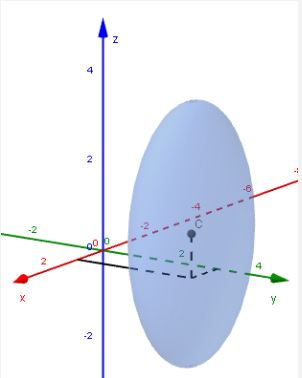
\includegraphics[width=6cm]{imagenes/Captura.jpg}
    \caption{Gráficas utilizando Geogebra para Elipsoide}
\end{figure}

\begin{figure}[hbtp]
    \centering
    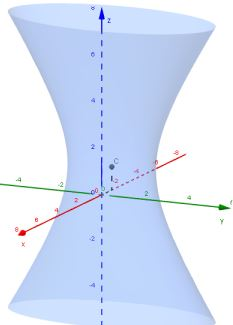
\includegraphics[width=6cm]{imagenes/Captura2.jpg}
    \caption{Gráficas utilizando Geogebra para Hiperboloide}
\end{figure}

\begin{tabular}{|c|c|c|c|}
    \hline
                 & Centrada en x & Centrada en y & Centrada en Z \\
    \hline
    Elipsoide    & 1             & 3             & 1             \\
    \hline
    Hiperboloide & -1            & 0             & 1             \\
    \hline
\end{tabular}
